\documentclass{beamer}
\usepackage[utf8]{inputenc}

\usetheme{Madrid}
\usecolortheme{default}
\usepackage{amsmath,amssymb,amsfonts,amsthm}
\usepackage{txfonts}
\usepackage{tkz-euclide}
\usepackage{listings}
\usepackage{adjustbox}
\usepackage{array}
\usepackage{tabularx}
\usepackage{gvv}
\usepackage{lmodern}
\usepackage{circuitikz}
\usepackage{tikz}
\usepackage{graphicx}

\setbeamertemplate{page number in head/foot}[totalframenumber]

\usepackage{tcolorbox}
\tcbuselibrary{minted,breakable,xparse,skins}



\definecolor{bg}{gray}{0.95}
\DeclareTCBListing{mintedbox}{O{}m!O{}}{%
  breakable=true,
  listing engine=minted,
  listing only,
  minted language=#2,
  minted style=default,
  minted options={%
    linenos,
    gobble=0,
    breaklines=true,
    breakafter=,,
    fontsize=\small,
    numbersep=8pt,
    #1},
  boxsep=0pt,
  left skip=0pt,
  right skip=0pt,
  left=25pt,
  right=0pt,
  top=3pt,
  bottom=3pt,
  arc=5pt,
  leftrule=0pt,
  rightrule=0pt,
  bottomrule=2pt,

  colback=bg,
  colframe=orange!70,
  enhanced,
  overlay={%
    \begin{tcbclipinterior}
    \fill[orange!20!white] (frame.south west) rectangle ([xshift=20pt]frame.north west);
    \end{tcbclipinterior}},
  #3,
}
\lstset{
    language=C,
    basicstyle=\ttfamily\small,
    keywordstyle=\color{blue},
    stringstyle=\color{orange},
    commentstyle=\color{green!60!black},
    numbers=left,
    numberstyle=\tiny\color{gray},
    breaklines=true,
    showstringspaces=false,
}
%------------------------------------------------------------
%This block of code defines the information to appear in the
%Title page
\title %optional
{5.2.31}
\date{september 2025}
%\subtitle{A short story}

\author % (optional)
{J.NAVYASRI- EE25BTECH11028}

\begin{document}

\frame{\titlepage}
\begin{frame}{Question:}
solve the following system of linear equations .
\[
2x + 3y  &= 8 \\
\]
\[
4x + 6y &= 7\\
\]
\end{frame}

\begin{frame}{Solution:}
Consider the system of linear equations:

\begin{equation}
2x + 3y = 8
\end{equation}

\begin{equation}
4x + 6y = 7
\end{equation}

\subsection*{Step 1: Write in matrix form}

\begin{equation}
\underbrace{\myvec{2 & 3 \\ 4 & 6}}_{\myvec{A}}
\underbrace{\myvec{x \\ y}}_{\myvec{X}}
=
\underbrace{\myvec{8 \\ 7}}_{\myvec{B}}
\end{equation}
\end{frame}

\begin{frame}{Solution:}
\subsection*{Step 2: Check the determinant of the coefficient matrix}

\begin{equation}
\det(A) = 
\begin{vmatrix} 2 & 3 \\ 4 & 6 \end{vmatrix} 
= (2)(6) - (3)(4) = 12 - 12 = 0
\end{equation}

Since the determinant is zero, the system is either inconsistent or has infinitely many solutions.

\subsection*{Step 3: Check for consistency}

Compare ratios of coefficients and constants:

\begin{equation}
\frac{2}{4} = \frac{3}{6} = \frac{1}{2} 
\quad \text{but} \quad 
\frac{8}{7} \neq \frac{1}{2}
\end{equation}

\subsection*{Conclusion}

The system is \textbf{inconsistent}. Therefore, 

\begin{equation}
\text{No solution exists.}
\end{equation}
\end{frame}


\begin{frame}[fragile]
    \frametitle{Python Code}
    \begin{lstlisting}
import numpy as np
import matplotlib.pyplot as plt

# Define x values
x = np.linspace(-5, 5, 400)

# Line 1: 2x + 3y = 8  => y = (8 - 2x)/3
y1 = (8 - 2*x)/3

# Line 2: 4x + 6y = 7  => y = (7 - 4*x)/6
y2 = (7 - 4*x)/6

# Plot the lines
plt.figure(figsize=(8,6))
plt.plot(x, y1, label='2x + 3y = 8', color='blue')
\end{lstlisting}
\end{frame}


\begin{frame}[fragile]
    \frametitle{Python Code}
    \begin{lstlisting}
plt.plot(x, y2, label='4x + 6y = 7', color='red', linestyle='--')

# Labels and grid
plt.xlabel('x')
plt.ylabel('y')
plt.title('Visualization of the system of equations')
plt.grid(True)
plt.axhline(0, color='black', linewidth=0.5)
plt.axvline(0, color='black', linewidth=0.5)
plt.legend()
plt.savefig("fig10.png")
plt.show()

\end{lstlisting}
\end{frame}


\begin{frame}{Plot-Using Python}
    \centering
    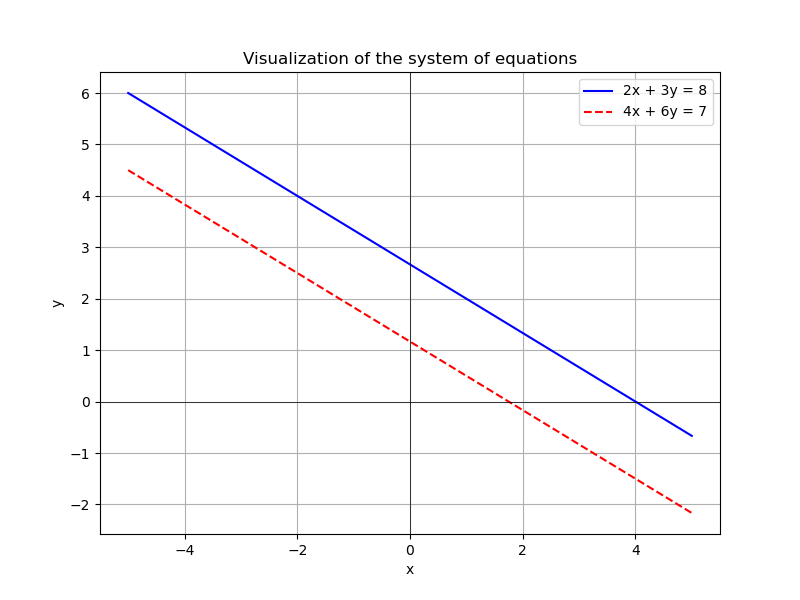
\includegraphics[width=\columnwidth, height=0.8\textheight, keepaspectratio]{figs/fig10.png}     
\end{frame}


\begin{frame}[fragile]
\frametitle{C Code}
\begin{lstlisting}
    #include <stdio.h>

int main() {
    // Coefficient matrix A
    double A[2][2] = {{2, 3}, {4, 6}};
    // Right-hand side vector B
    double B[2] = {8, 7};

    // Compute determinant
    double det = A[0][0]*A[1][1] - A[0][1]*A[1][0];

    if(det != 0) {
        // If determinant is non-zero, solve using Cramer's rule
        double x = (B[0]*A[1][1] - B[1]*A[0][1]) / det;
        double y = (A[0][0]*B[1] - A[1][0]*B[0]) / det;
        \end{lstlisting}

\end{frame}

\begin{frame}[fragile]
\frametitle{C Code}
\begin{lstlisting}
        printf("Unique solution:\n");
        printf("x = %.2lf\n", x);
        printf("y = %.2lf\n", y);
    } else {
        // Determinant is zero, check for consistency
        if((A[0][0]*B[1] - A[1][0]*B[0] != 0) || (A[0][1]*B[1] - A[1][1]*B[0] != 0)) {
            printf("The system is inconsistent. No solution exists.\n");
        } else {
            printf("The system has infinitely many solutions.\n");
        }
    }

    return 0;
}
  \end{lstlisting}

\end{frame}


\begin{frame}[fragile]
\frametitle{Python and C Code}

\begin{lstlisting}
import ctypes
import numpy as np
import matplotlib.pyplot as plt

# Load the C library
lib = ctypes.CDLL("./linear.so")

# Define array size
n = 400
x = np.linspace(-10, 10, n)
\end{lstlisting}

\end{frame}


\begin{frame}[fragile]
\frametitle{Python and C Code}

\begin{lstlisting}
# Create empty arrays for y1, y2
y1 = np.zeros(n, dtype=np.double)
y2 = np.zeros(n, dtype=np.double)

# Convert numpy arrays to ctypes pointers
lib.compute_lines.argtypes = [np.ctypeslib.ndpointer(dtype=np.double, ndim=1, flags="C_CONTIGUOUS"),
                              np.ctypeslib.ndpointer(dtype=np.double, ndim=1, flags="C_CONTIGUOUS"),
                              np.ctypeslib.ndpointer(dtype=np.double, ndim=1, flags="C_CONTIGUOUS"),
                              ctypes.c_int]

lib.compute_lines(x, y1, y2, n)
\end{lstlisting}

\end{frame}


\begin{frame}[fragile]
\frametitle{Python and C Code}

\begin{lstlisting}

# Plot the results
plt.plot(x, y1, label="2x + 3y - 8 = 0")
plt.plot(x, y2, label="4x + 6y - 7 = 0")
plt.xlabel("x")
plt.ylabel("y")
plt.title("Plot using C computations via ctypes")
plt.grid(True)
plt.legend()
plt.show()
\end{lstlisting}

\end{frame}

\begin{frame}{Plot-Using by C and Python}
    \centering
    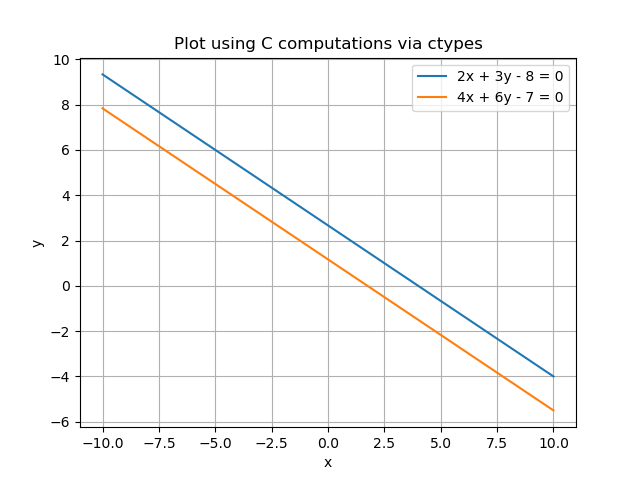
\includegraphics[width=\columnwidth, height=0.8\textheight, keepaspectratio]{figs/fig10.1.png}     
\end{frame}
\end{document}
